\documentclass[a4paper,11pt,UTF8]{article}
\usepackage{ctex}
\usepackage{amsmath,amsthm,amssymb,amsfonts}
\usepackage{amsmath}
\usepackage[a4paper]{geometry}
\usepackage{graphicx}
\usepackage{microtype}
\usepackage{siunitx}
\usepackage{booktabs}
\usepackage[colorlinks=false, pdfborder={0 0 0}]{hyperref}
\usepackage{cleveref}
\usepackage{esint} 
\usepackage{graphicx}
\usepackage{ragged2e}
\usepackage{pifont}
\usepackage{extarrows}
\usepackage{mathptmx}
\usepackage{float}
\usepackage{caption}
\usepackage{multirow}
\usepackage{subfigure}
\usepackage{titlesec}
\titleformat{\section}{\Large\bfseries}{\chinese{section}、}{0em}{}
\titleformat{\subsection}{\large\bfseries}{}{0em}{}
\titleformat{\subsubsection}{\normalsize\bfseries}{}{1em}{}
\begin{document}
	
\begin{titlepage}
	\begin{center}
		\vspace*{1cm}
		\textbf{\LARGE 实验报告:集成运算放大器在信号运算方面的应用}
		
		\vspace{0.5cm}
		\Large 谢悦晋\quad 提高2201班\quad U20221033
		
		\vspace{1cm}
		\begin{figure}[H]
			\centering
			\subfigure{
				
\includegraphics[scale=1]{hust}
			}
			\subfigure{
				
\includegraphics[scale=1]{eic}
			}
			\caption*{}
		\end{figure}
		\vfill
		
		
		\vspace{0.8cm}
		华中科技大学 \\
		电子信息与通信学院 \\
		Oct 22nd, 2023
	\end{center}
\end{titlepage}

\section{实验目的}
熟练安装、调试本节介绍的由运放构成的基本运算电路,熟练掌握它们的工作原理,掌握运放电路的基本分析
\section{实验器材}
运算放大器NE5532,100$\mathrm{\Omega}$电阻,500$\mathrm{\Omega}$电阻,1$\mathrm{k\Omega}$电阻,5.1$\mathrm{k\Omega}$电阻,10$\mathrm{k\Omega}$电阻,100$\mathrm{k\Omega}$电阻,示波器,信号源,稳压电源
\section{实验内容}
\subsection{任务1: 研究电压跟随器的作用}
测试下图所示两种电路各电压幅值,观察有、无电压跟随器的差别。
\subsubsection{实验电路:}
\begin{figure}[H]
	\centering
	\setcounter{subfigure}{0}
	\subfigure[直接连接]{
		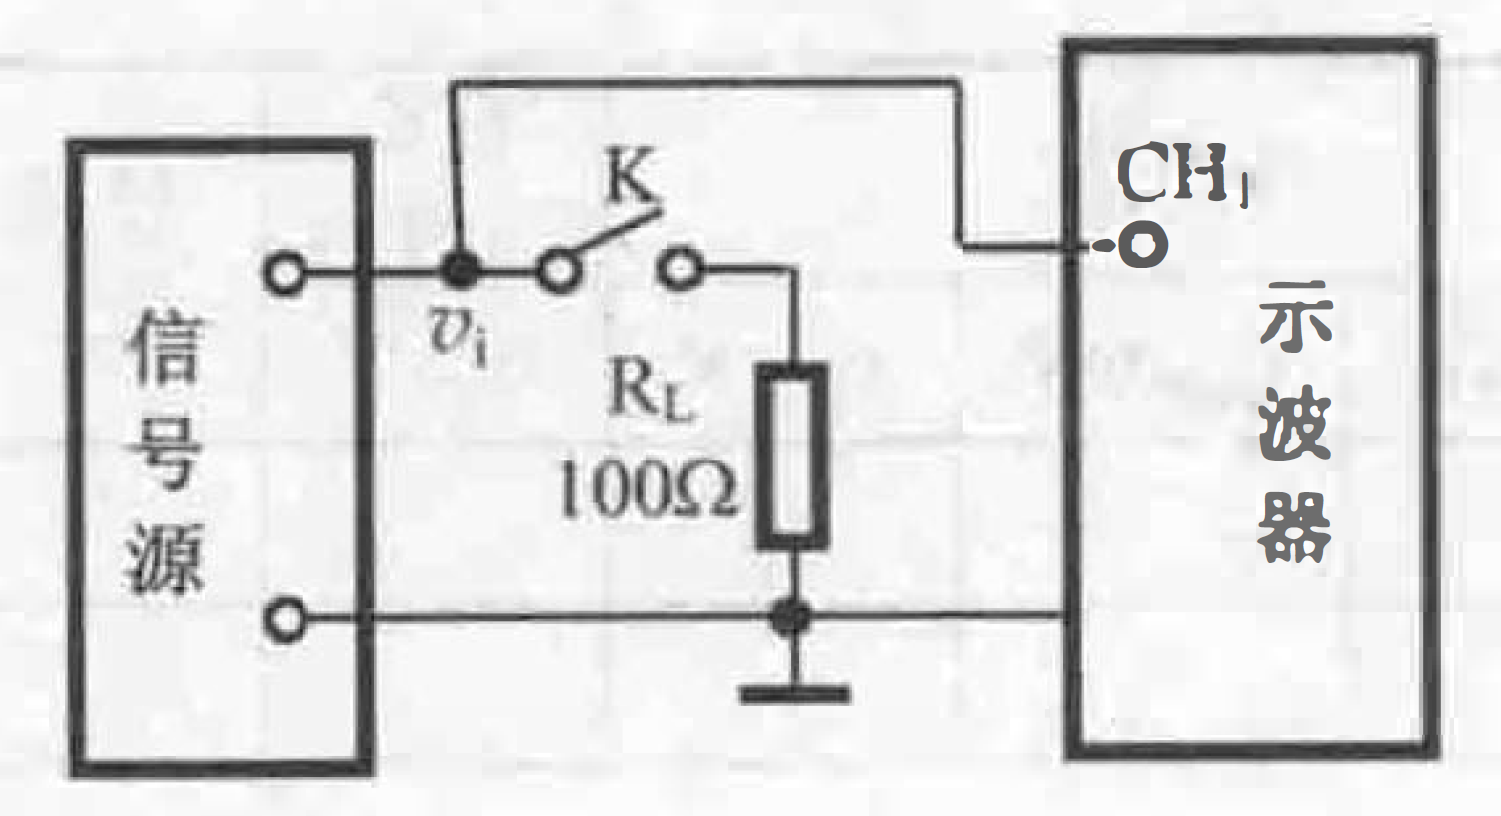
\includegraphics[scale=0.1]{1.1}
		\label{fig:subfig1}		
	}
	\subfigure[通过电压跟随器连接]{
		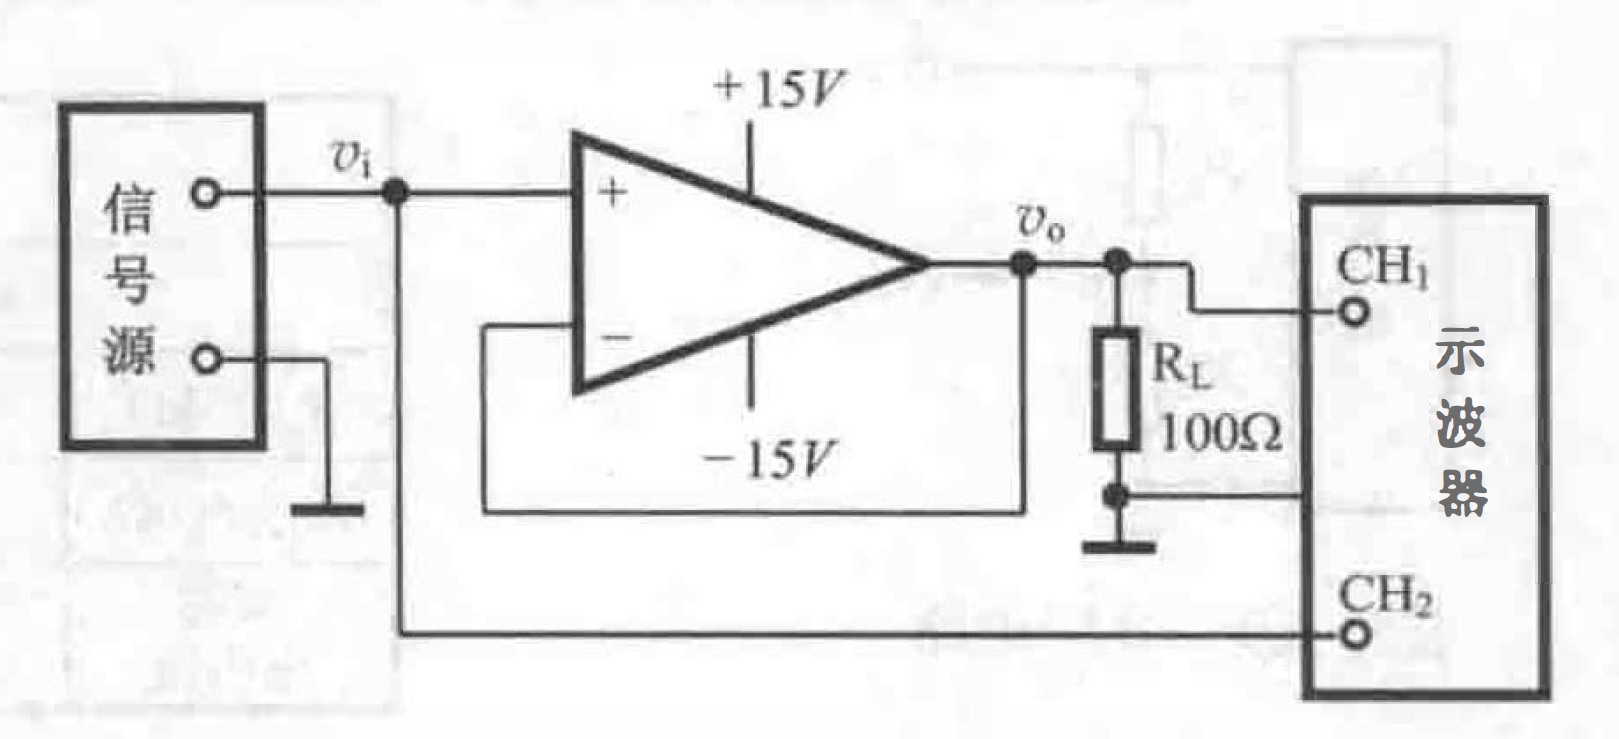
\includegraphics[scale=0.12]{1.2}
	}
	\caption*{任务1: 研究电压跟随器的作用}
\end{figure}
信号源的内阻计算可以按照分压公式计算:
$$
	R_s=\frac{V_s-v_{ipp(R_L)}}{v_{ipp(R_L)}}R_L
$$
观察到的波形如下:
\begin{figure}[H]
	\centering
	\setcounter{subfigure}{0}
	\subfigure[不接入$R_L$]{
		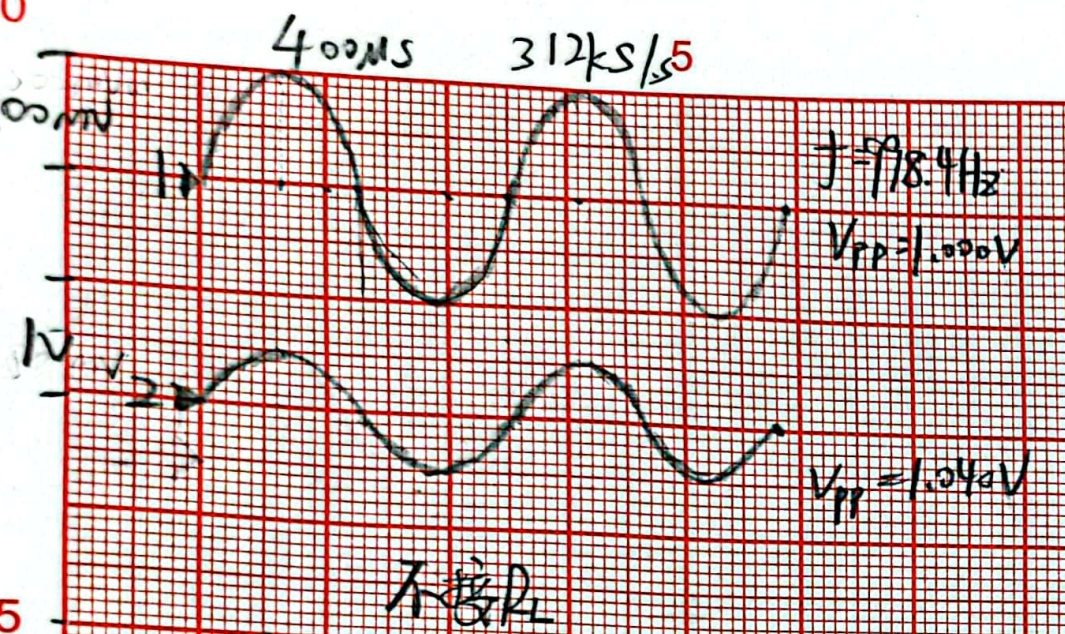
\includegraphics[scale=0.049]{1.7}
	}
	\subfigure[接入$R_L$]{
		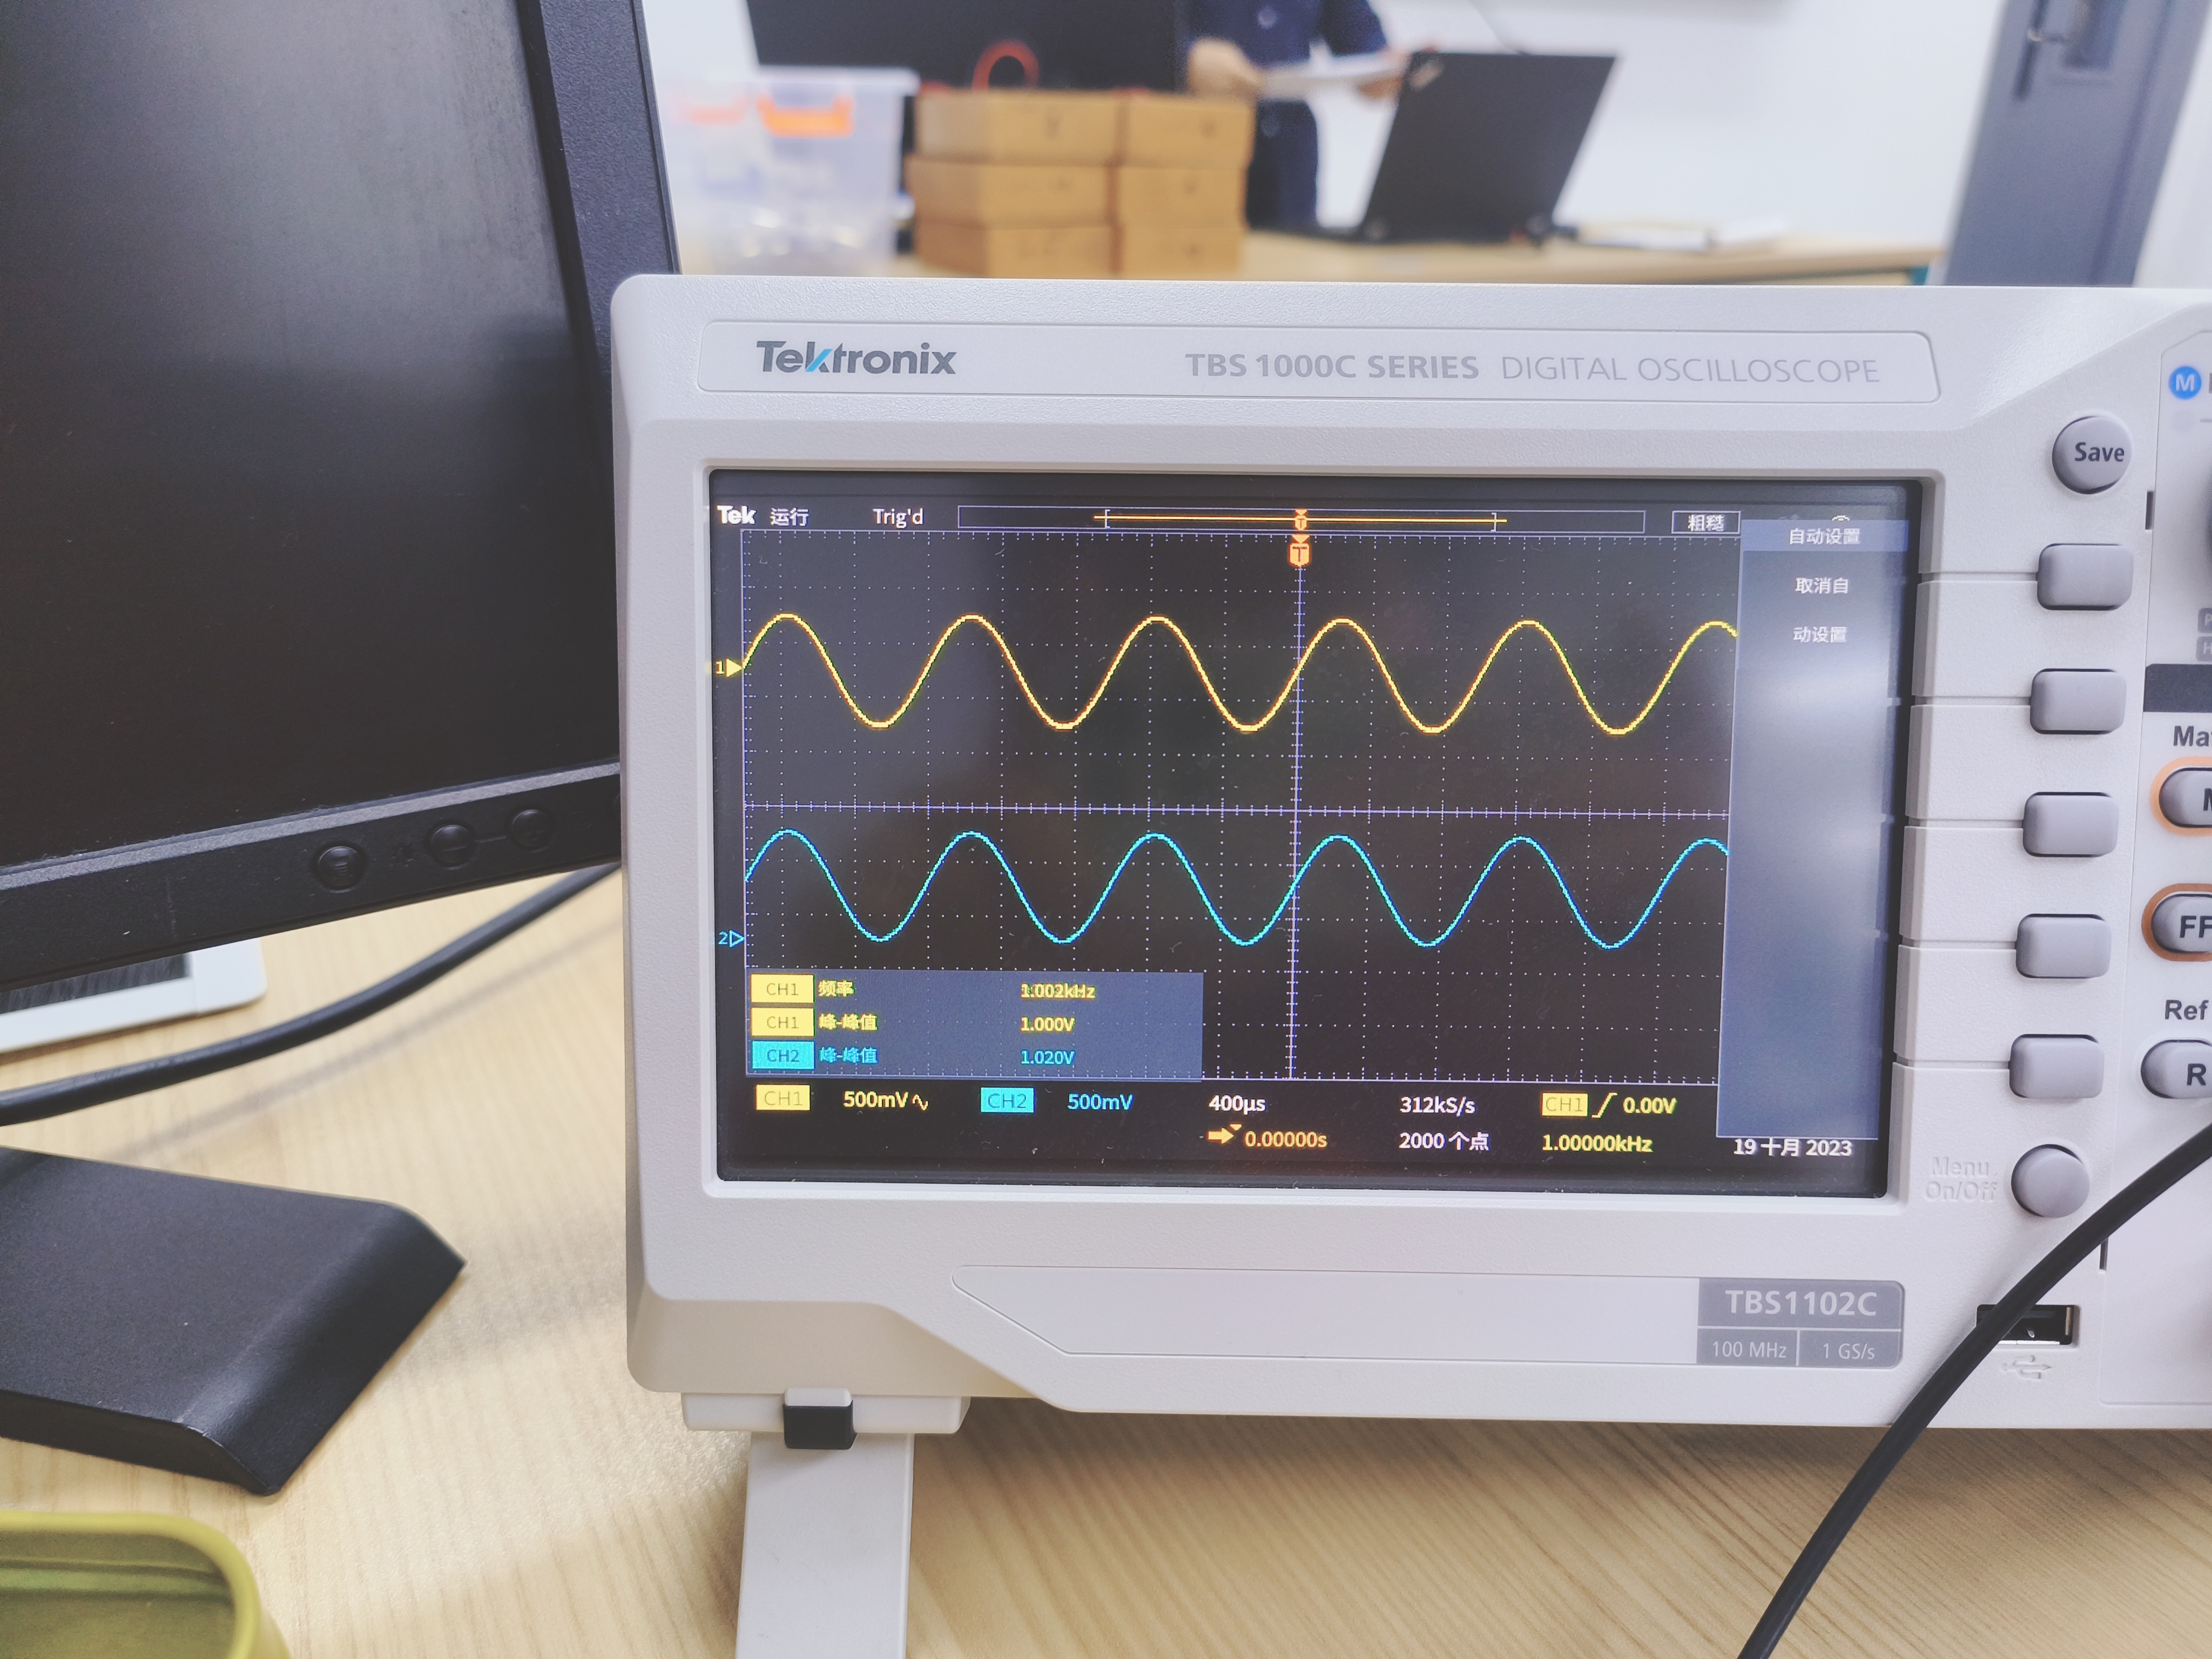
\includegraphics[scale=0.049]{1.8}
	}

	\caption*{无信号跟随器}
\end{figure}
\begin{figure}[H]
	\centering
	\setcounter{subfigure}{0}
	\subfigure[不接入$R_L$]{
		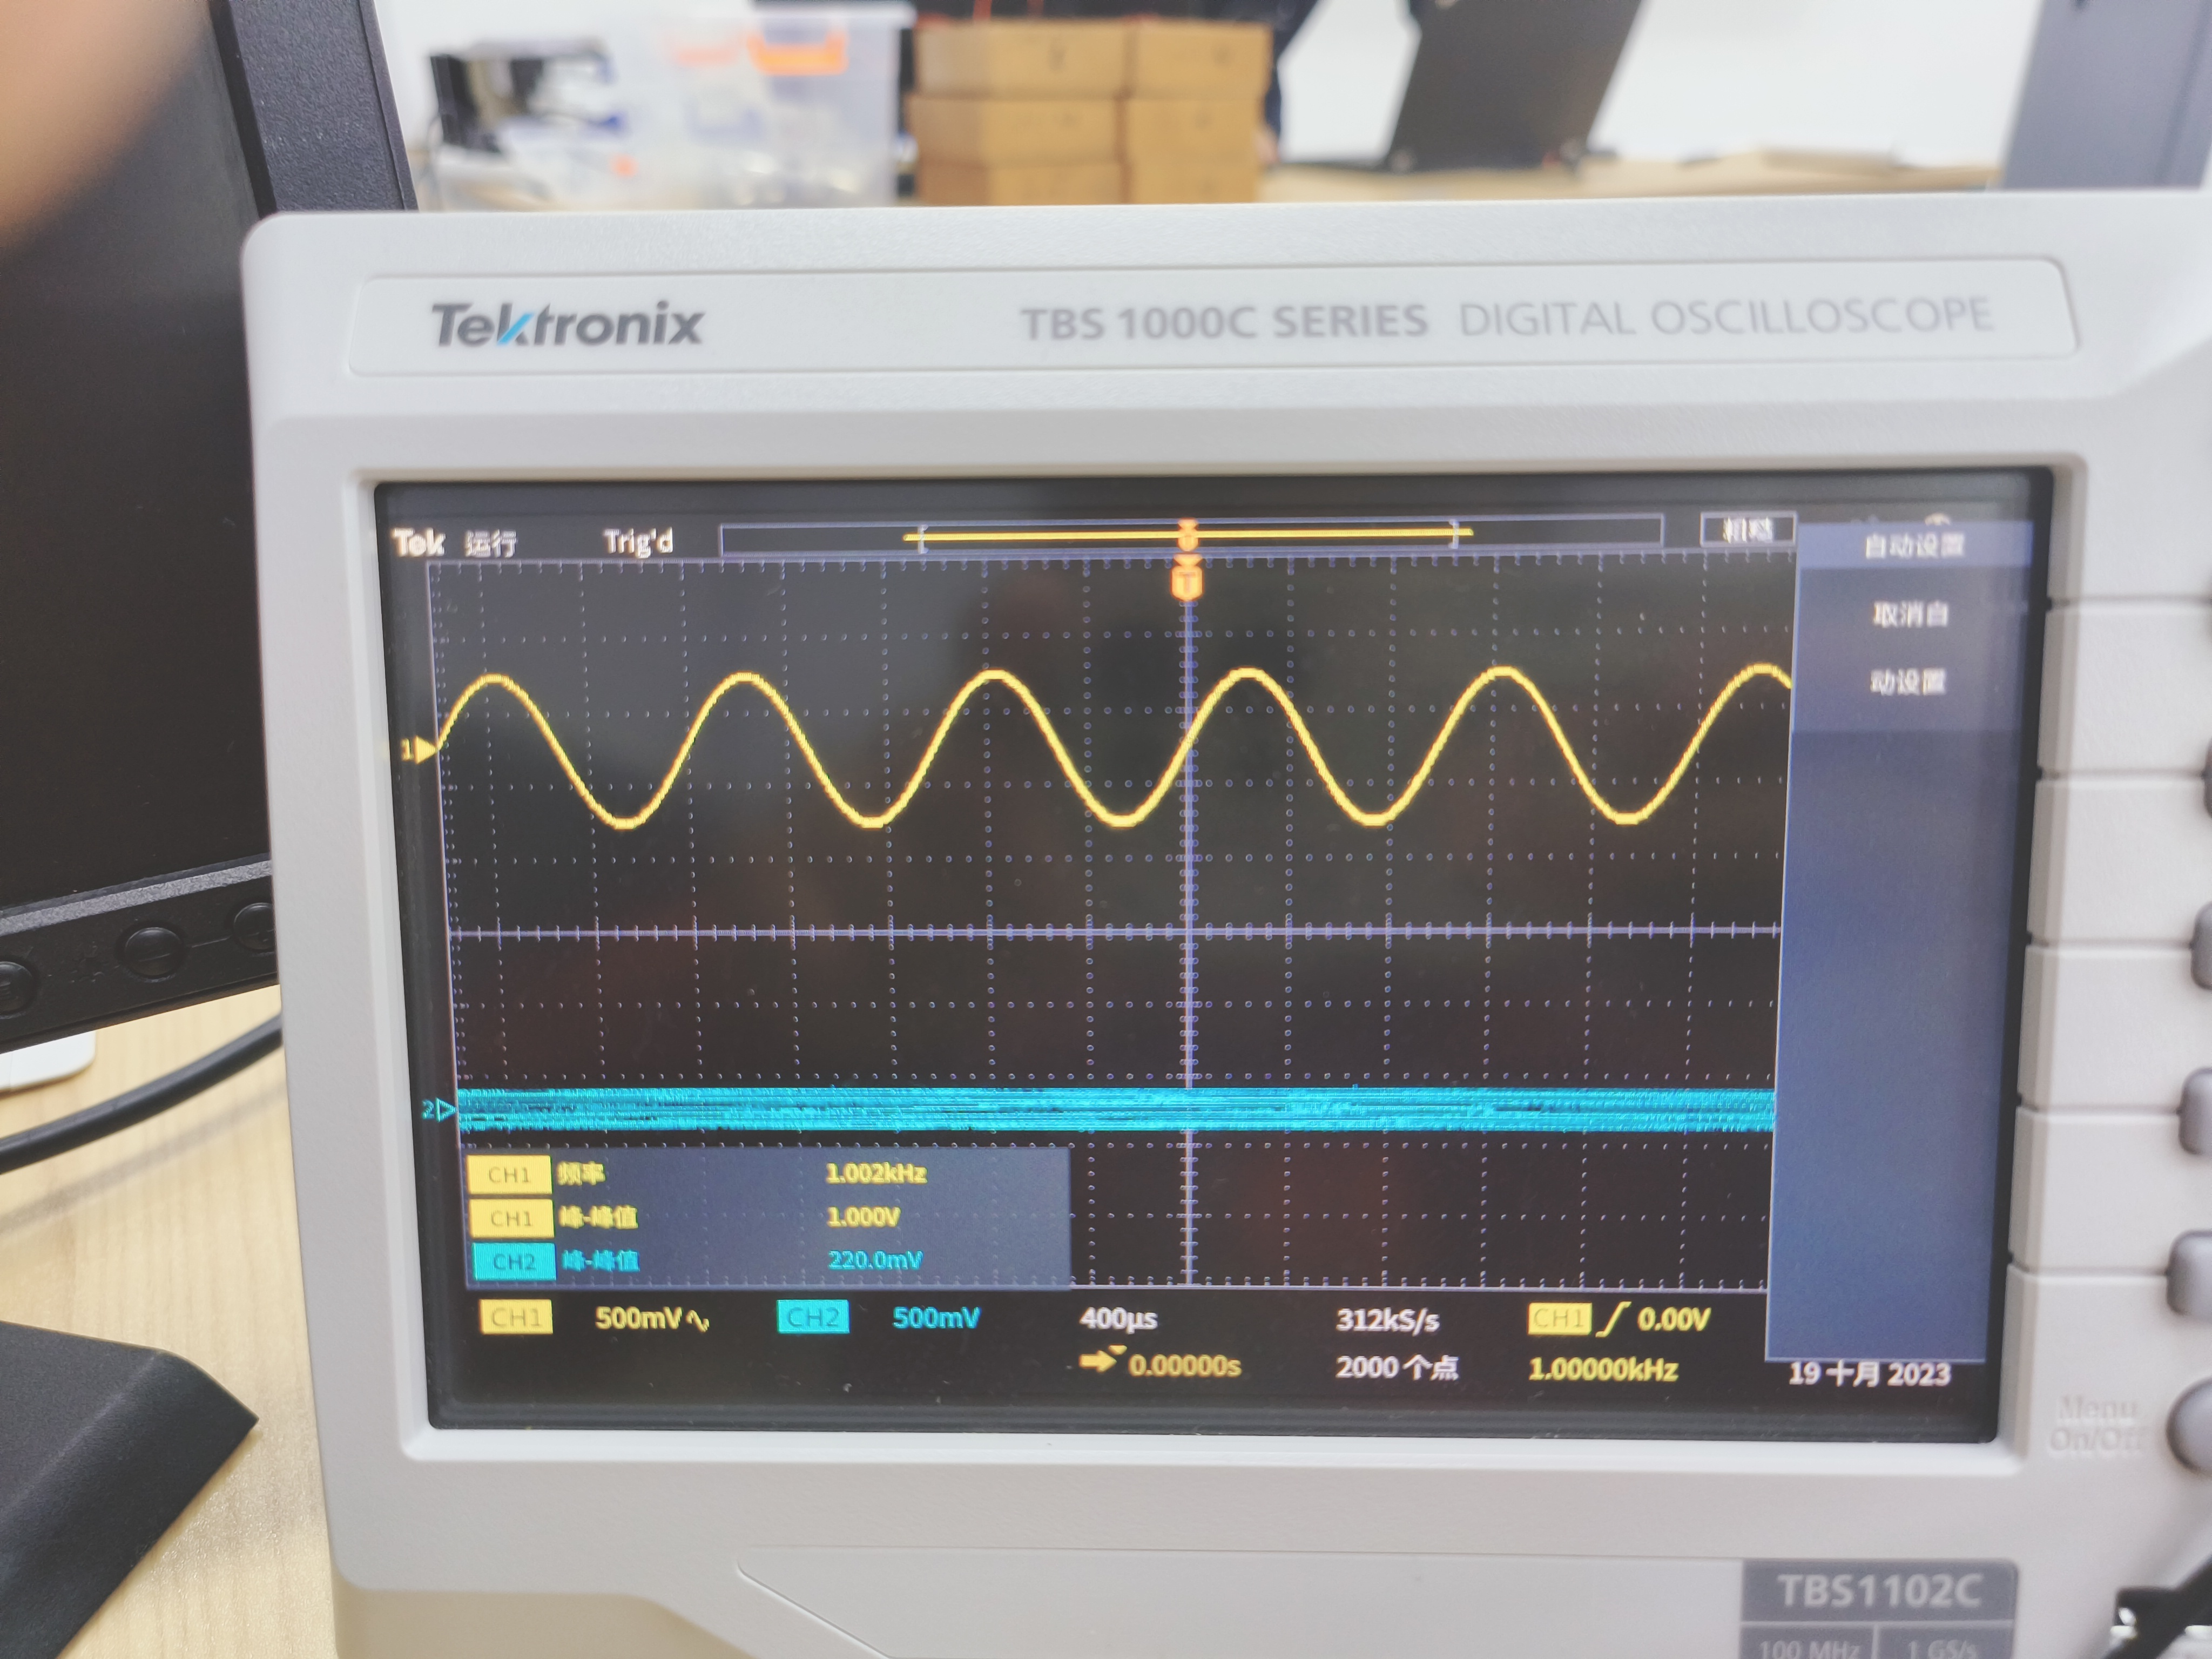
\includegraphics[scale=0.049]{1.5}
	}
	\subfigure[接入$R_L$]{
		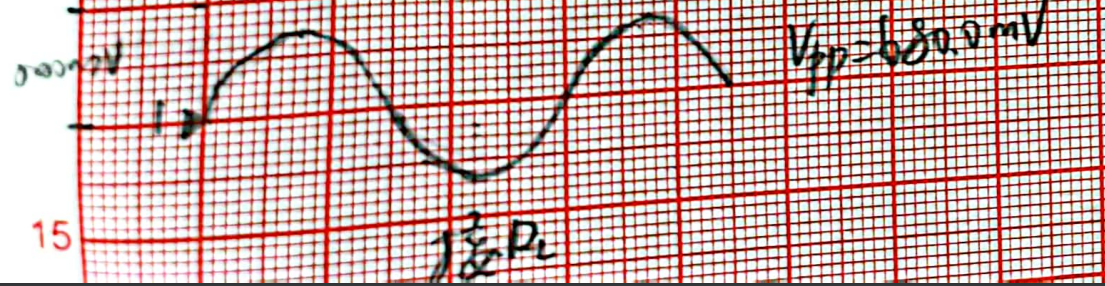
\includegraphics[scale=0.049]{1.6}
	}
	
	\caption*{有信号跟随器}
\end{figure}

\begin{table*}[h]
	\centering
	\caption*{电压跟随器的作用}

	\begin{tabular}{|c|c|c|c|c|c|}
		\hline
		\multirow{2}{*}{}   & \multicolumn{2}{c|}{不接$R_L$} & \multicolumn{2}{c|}{接入$R_L$} &
		\multirow{2}{*}{计算$R_s/\Omega$}\\
		\cline{2-5}
		\multirow{2}{*}{} & $v_{ipp}/$V & $v_{opp}/$V & $v_{ipp}/$V & $v_{opp}/$V & \multirow{2}{*}{}\\
		\hline
		无电压跟随器 & 1.000 & - & 0.6800 & - & 47.06\\
		\hline
		有电压跟随器 & 1.000 & 1.020 & 1.000 & 1.040 & - \\
		\hline
	\end{tabular}
	\label{table_MAP}
\end{table*}



\subsection{任务2: 反相比例加法运算电路测试}
测试图3.6.8所示反相比例加法器的输入输出电压,验证它们的运算关系。根据运放的虚短和虚断特性,可求得其输出电压为:
$$
	V_0=-\left(\frac{R_{\mathrm{F}}}{R_1}V_1+\frac{R_{\mathrm{F}}}{R_2}V_2\right)
$$
\subsubsection{实验电路:}
\begin{figure}[H]
	\centering
	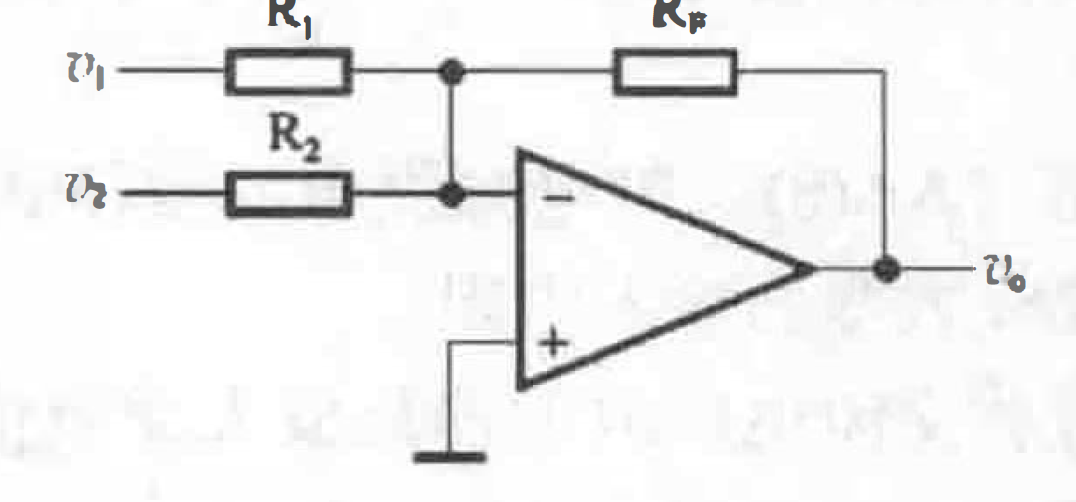
\includegraphics[scale=0.2]{1.3}
	\caption*{任务2: 反相比例加法运算电路测试}
\end{figure}
\begin{table*}[h]
	\centering
	\caption*{加法器}
	\label{table1}
	\begin{tabular}{|c|c|c|c|c|c|}
		\hline
		\multirow{2}{*}{}   & \multicolumn{3}{c|}{实测值} & 理论值 &
		\multirow{2}{*}{相对误差}\\
		\cline{2-5}
		\multirow{2}{*}{} & $v_{1pp}$/V & $v_{2pp}/$/V & $v_{opp}$/V & $v_{opp}$/V & \multirow{2}{*}{}\\
		\hline
		$R_{s2}=1\mathrm{k\Omega}$ & & & & &\\
		\hline
		$R_{s2}=500\mathrm{\Omega}$ & \multicolumn{5}{c|}{$R_1=,R_2=, R_F=$}\\
		\hline
	\end{tabular}
\end{table*}
\begin{figure}[H]
	\centering
	\setcounter{subfigure}{0}
	\subfigure[$v_{1pp}$]{
		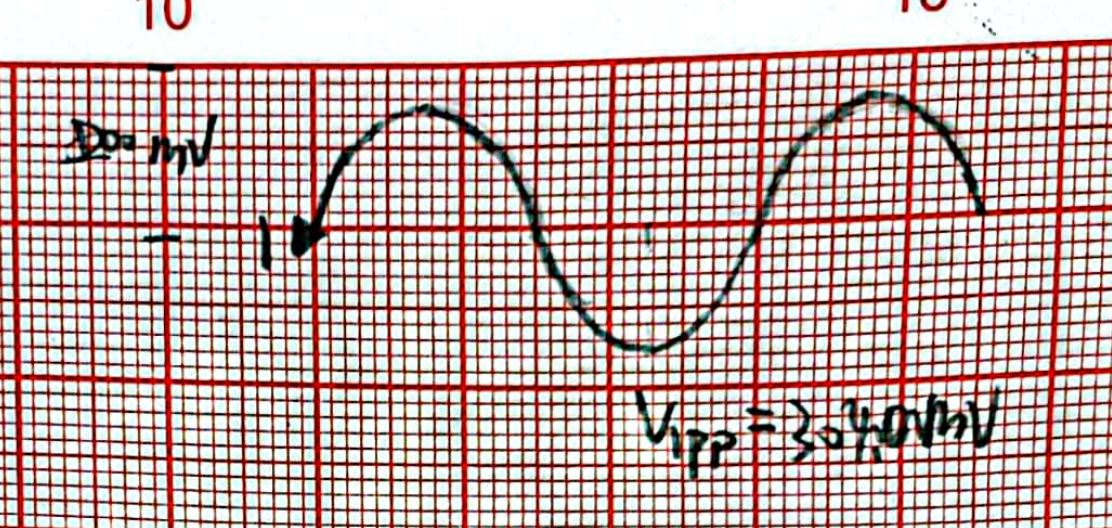
\includegraphics[scale=0.049]{1.9}
	}
	\subfigure[$v_{2pp}$]{
		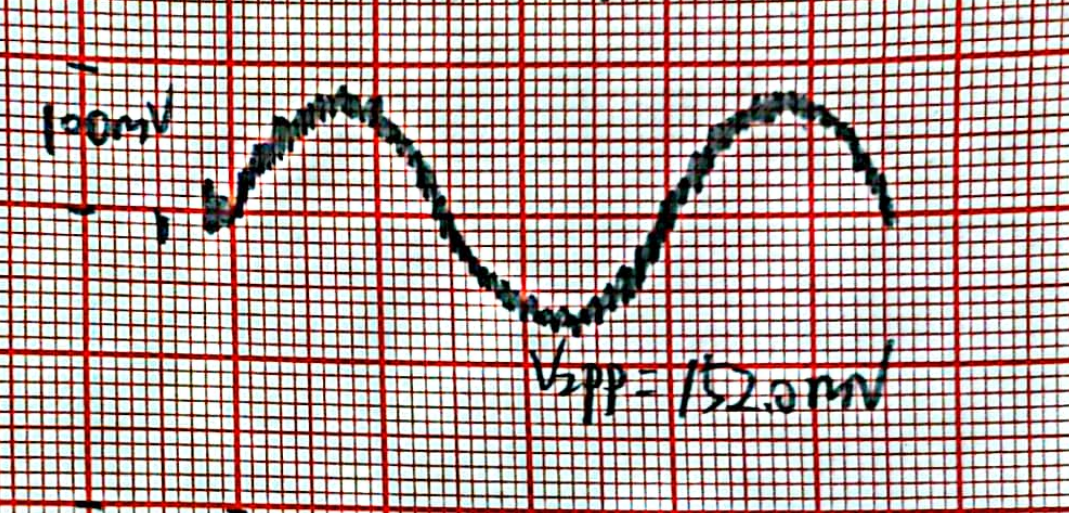
\includegraphics[scale=0.049]{1.10}
	}
	\subfigure[$v_{opp}$]{
		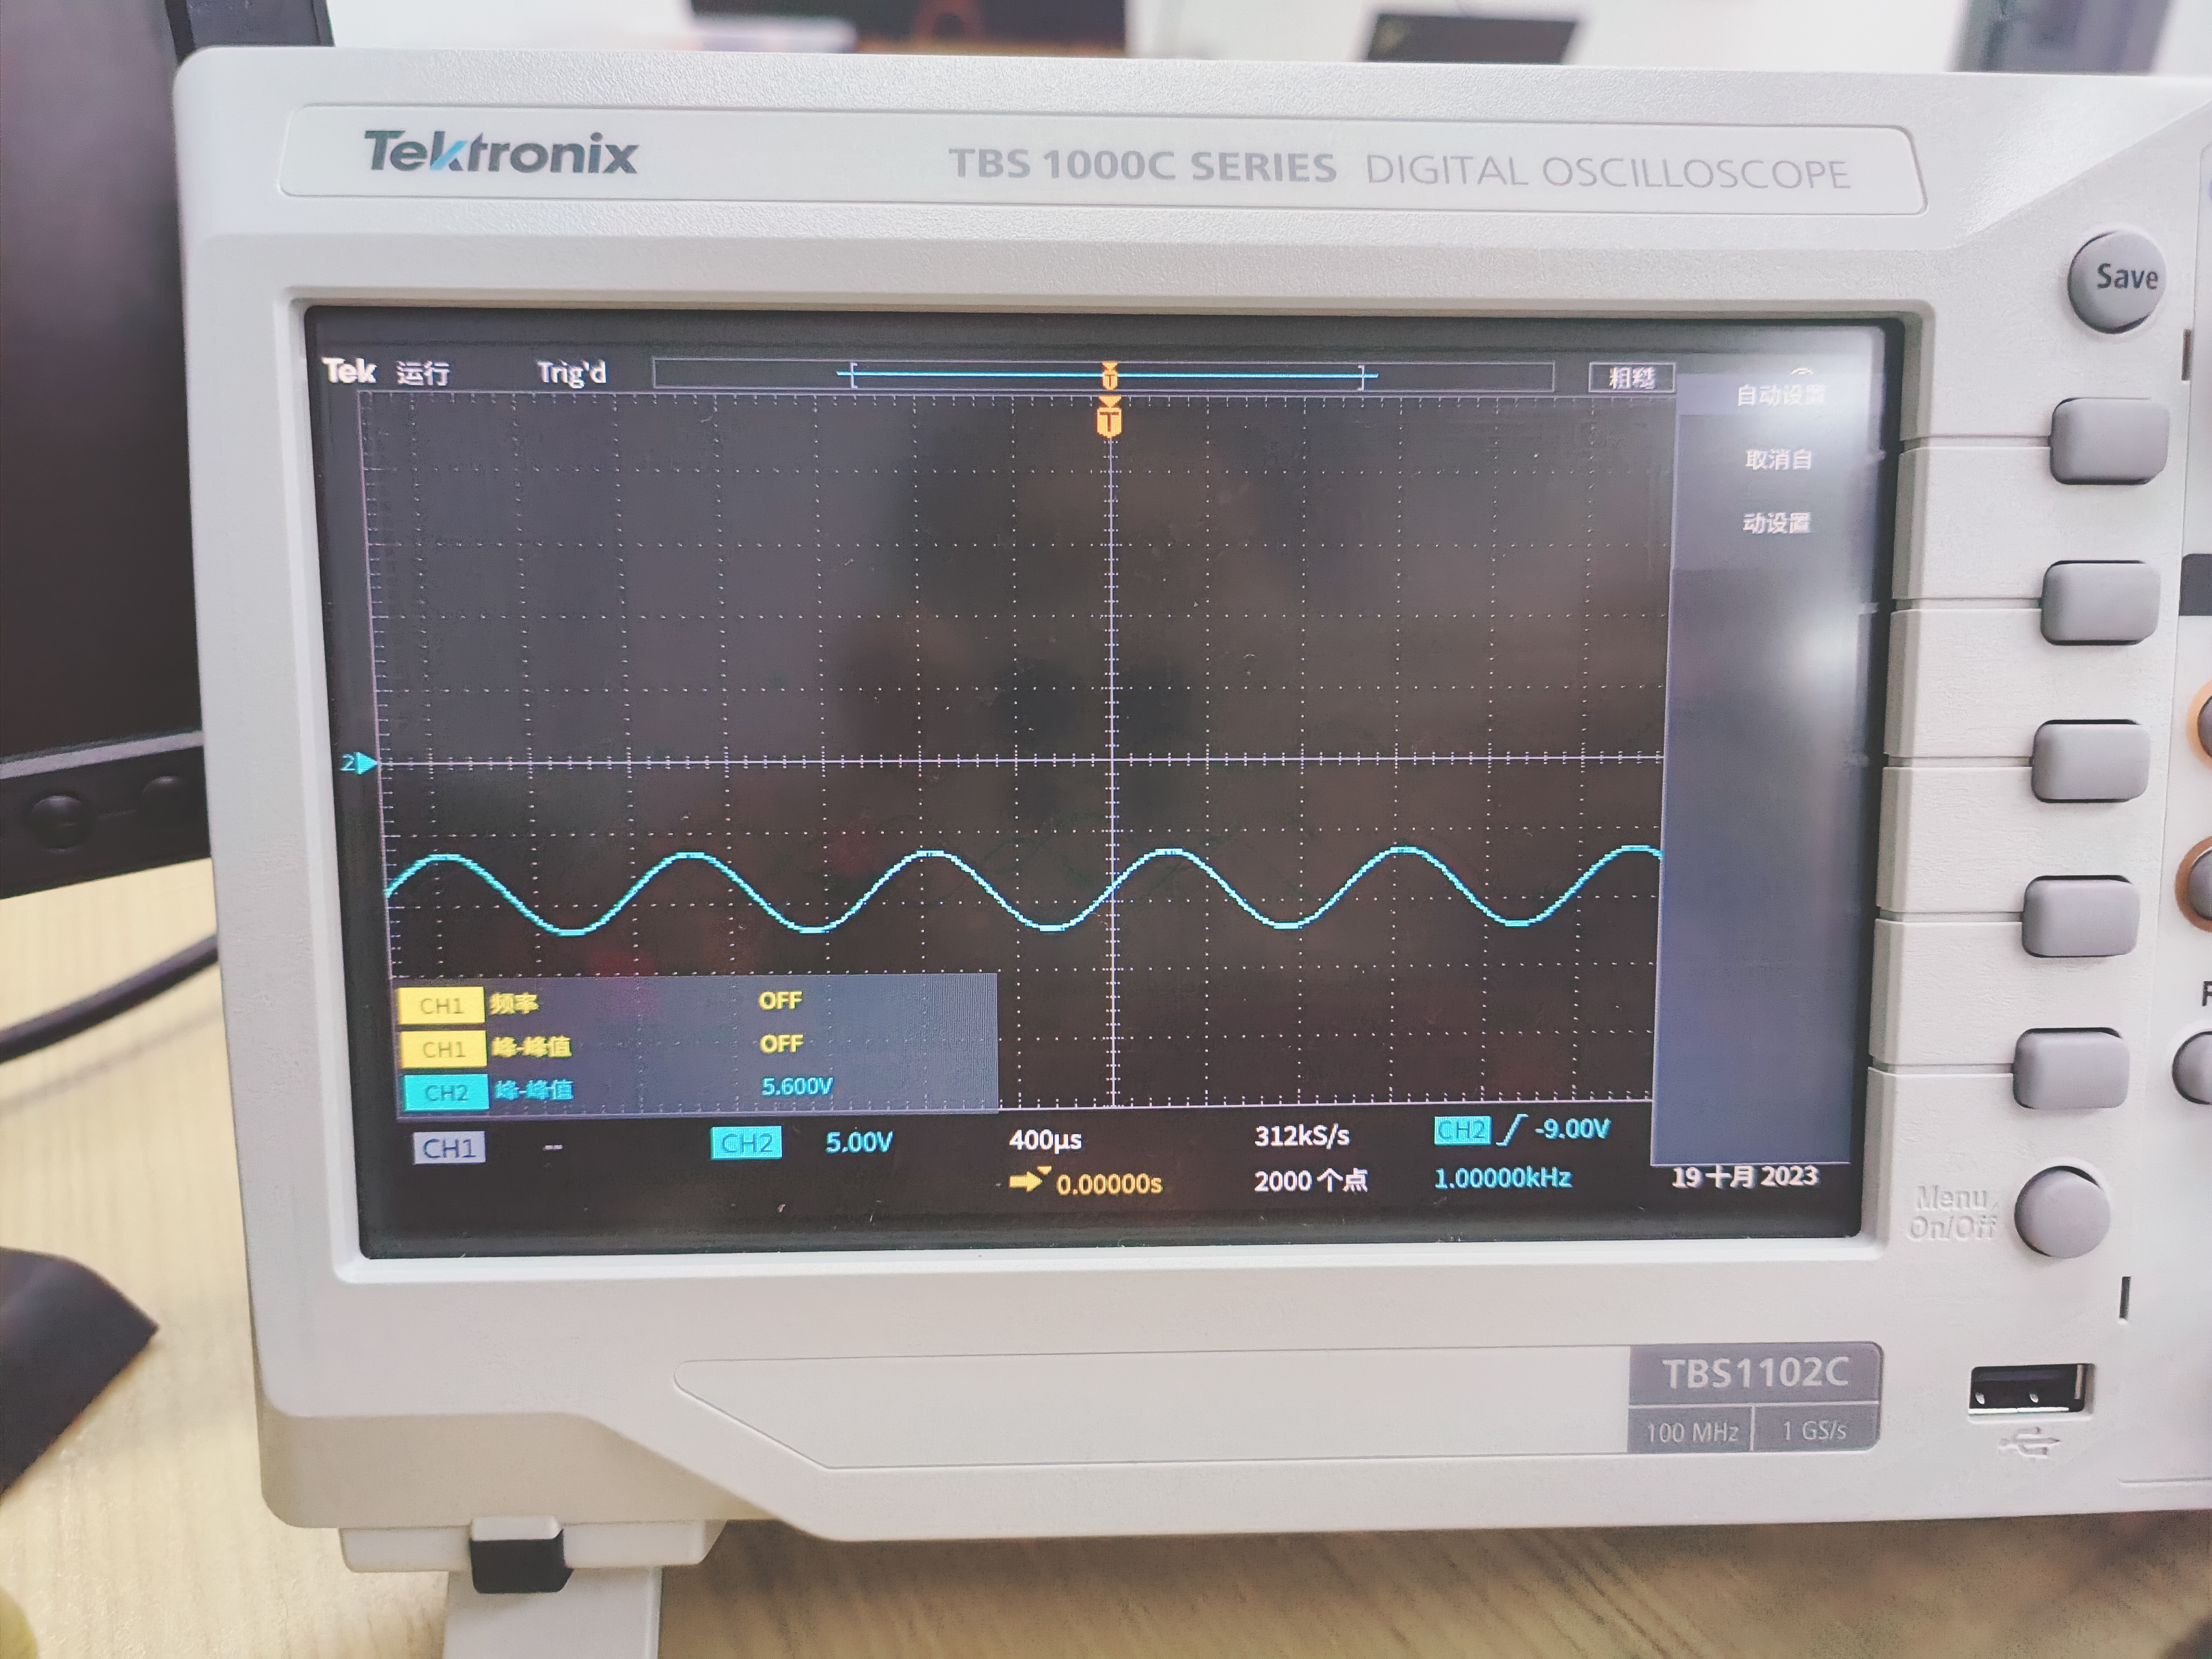
\includegraphics[scale=0.049]{1.11}
	}
	\caption*{无信号跟随器}
\end{figure}
\subsection{任务3: 比例积分电路测试}
测试图3.6.10所示比例积分器的输入、输出波形。 当$R_F\gg R_1$时,电路的输出电压可近似为:
$$
	v_{\mathrm{o}}(t)=-\frac{1}{R_{1}C}\int_{0}^{t}v_{\mathrm{i}}(t)\mathrm{d}t+v_{\mathrm{o}}(0)
$$
\subsubsection{实验电路:}
\begin{figure}[H]
	\centering
	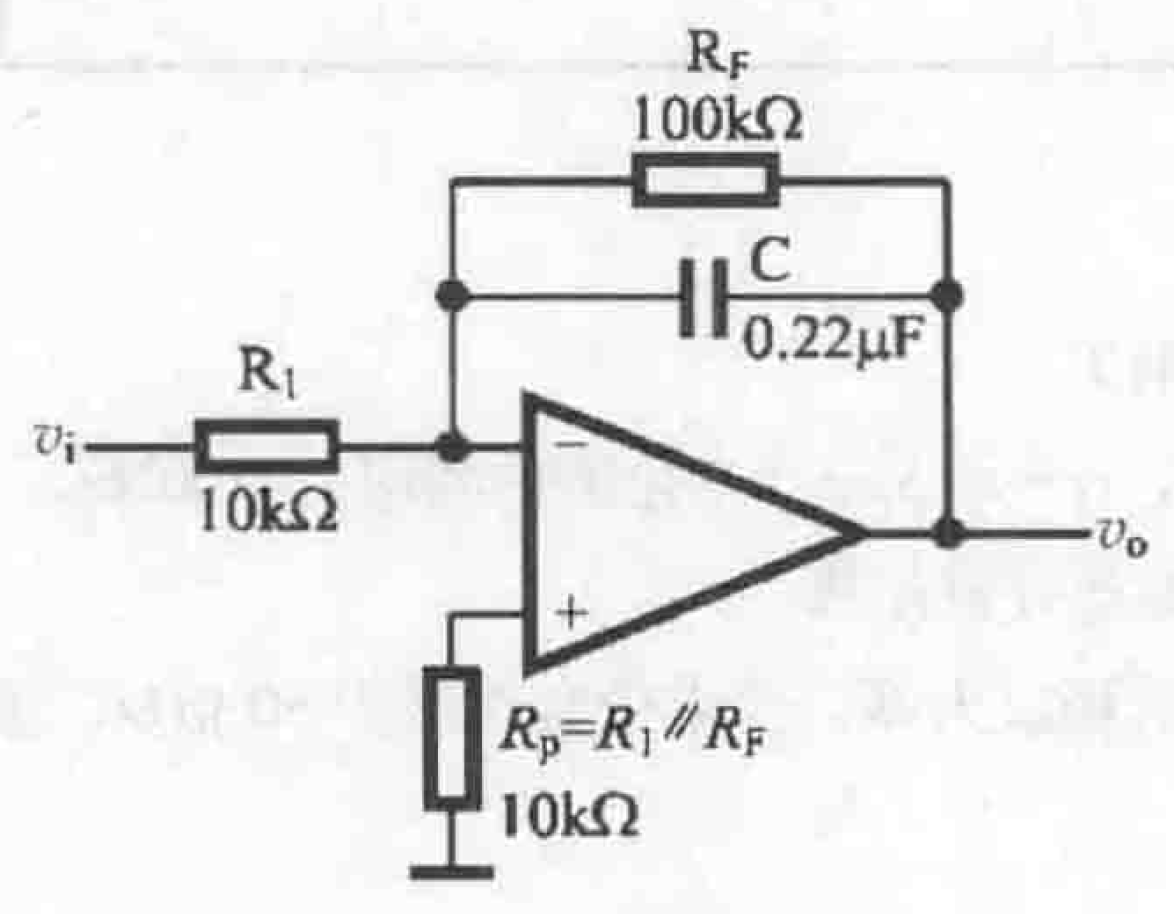
\includegraphics[scale=0.18]{1.4}
	\caption*{任务3: 比例积分电路测试}
\end{figure}
\begin{figure}[H]
	\centering
	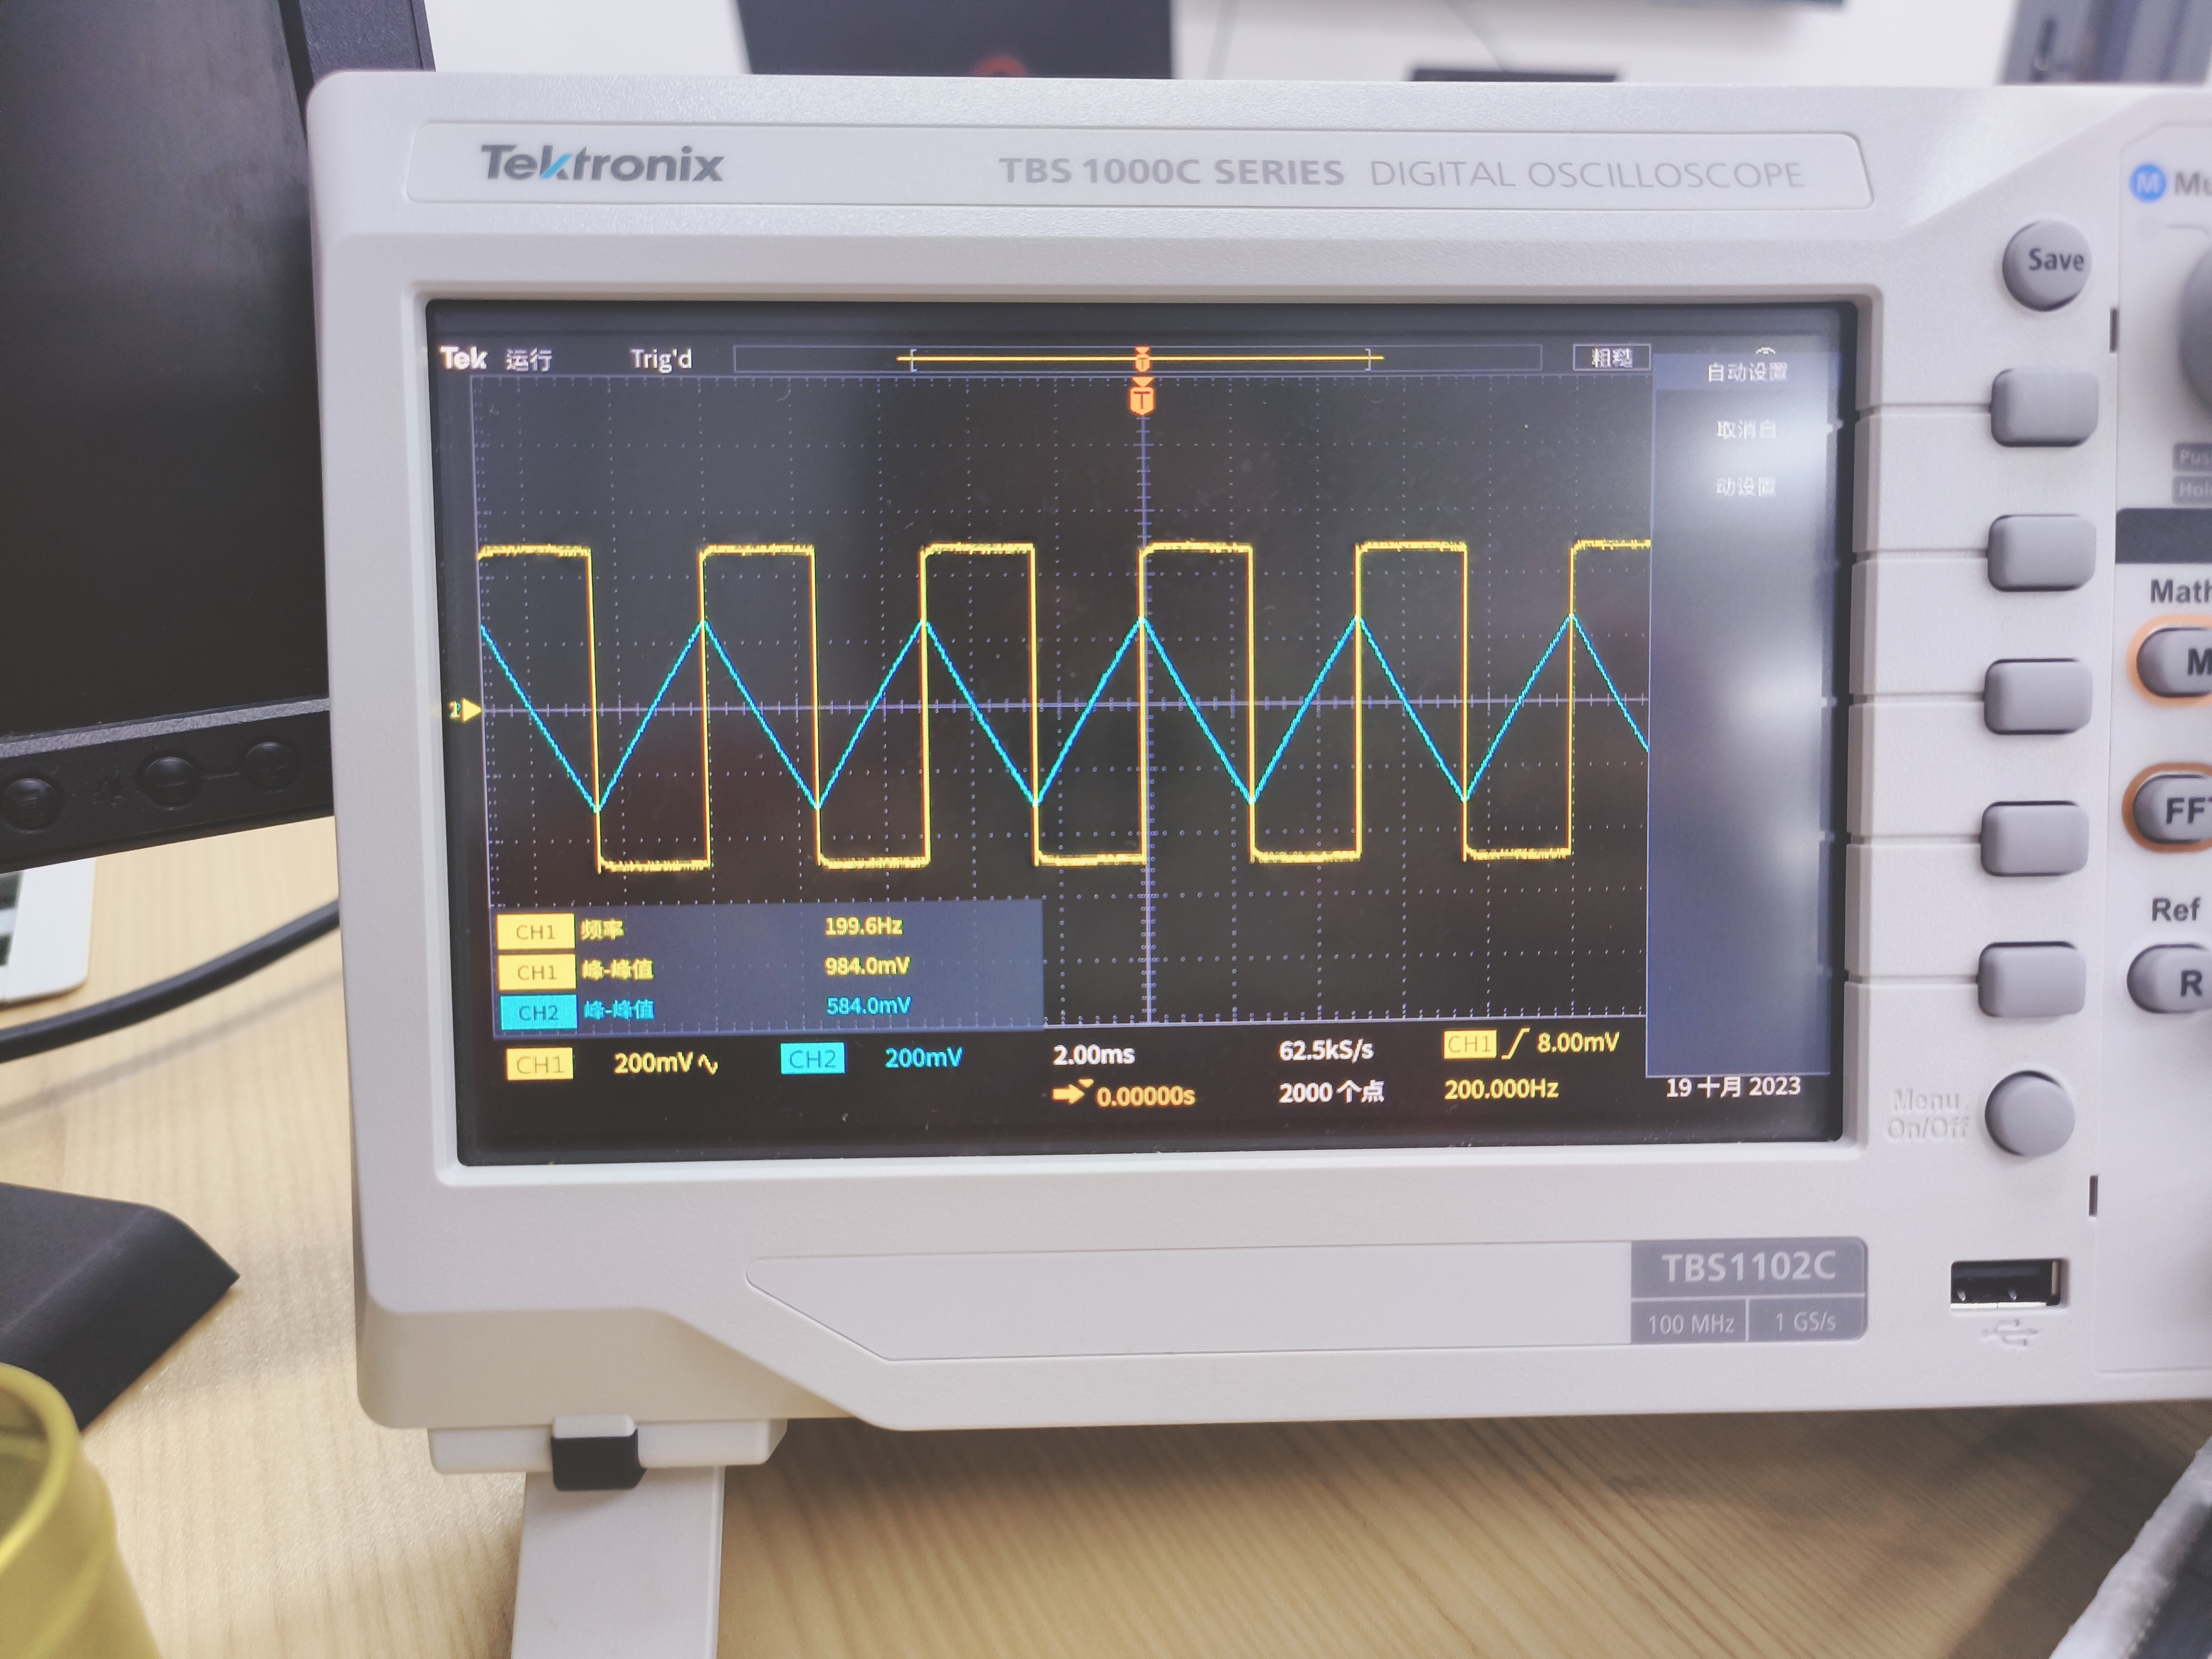
\includegraphics[width=0.7\textwidth]{1.12}
	\caption*{比例积分电路}
\end{figure}
\end{document}